\documentclass[12pt,prb,aps,epsf]{article}
\usepackage[utf8]{inputenc}
\usepackage{amsmath}
\usepackage{amsfonts}
\usepackage{amssymb}
\usepackage{graphicx} 
\usepackage{latexsym} 
\usepackage[toc,page]{appendix}
\usepackage{listings}
\usepackage{xcolor}
\usepackage{soul}
\usepackage[T1]{fontenc}
\usepackage{amsthm}
\usepackage{mathtools}
\usepackage{setspace}
\usepackage{array,multirow,makecell}
\usepackage{geometry}
\usepackage{textcomp}
\usepackage{float}
%\usepackage{siunitx}
\usepackage{cancel}
%\usepackage{tikz}
%\usetikzlibrary{calc, shapes, backgrounds, arrows, decorations.pathmorphing, positioning, fit, petri, tikzmark}
\usepackage{here}
\usepackage{titlesec}
%\usepackage{bm}
\usepackage{bbold}
\geometry{hmargin=2cm,vmargin=2cm}

\begin{document}
	
	\title{LP 12 Rayonnement d'équilibre thermique, corps noir}
		\author{Naïmo Davier}
		\date{Agrégation 2019}
		
	\maketitle
	
	\tableofcontents
	
	\pagebreak
	
Niveau L3

En introduction manip : transfert de chaleur par rayonnement : on fait chauffer une thermopile avec une lampe à quartz.\\
donner la formule de Planck au milieu de la leçon, la discuter puis la démontrer à la fin.
	
	
\section{Rayonnement thermique}
\subsection{Transport d'énergie, définitions}
Lien avec l'électromag : $\vec{E}(\vec{k},\vec{\alpha}) = \vec{\alpha}e^{i(\vec{k}.\vec{r}-\omega t)}$ : il y a deux polarisations transverses.\\ 
On définit les grandeurs $\vec{k},\,c,\,\omega,\,\lambda$.\\
Energie transmise par le rayonnement, emittance radiative : quantité d'énergie mesurée par unité de temps et de surface.
\begin{eqnarray}
\varepsilon = \int e(\nu)d\nu
\end{eqnarray}
avec $e(\nu)$ l'emittance spectrale.
\begin{eqnarray}
E_{tot} = \int dS \int_0^{\tau} dt \varepsilon
\end{eqnarray}

\subsection{Rayonnement d'équilibre thermique}
\begin{figure}[h]
	\centering 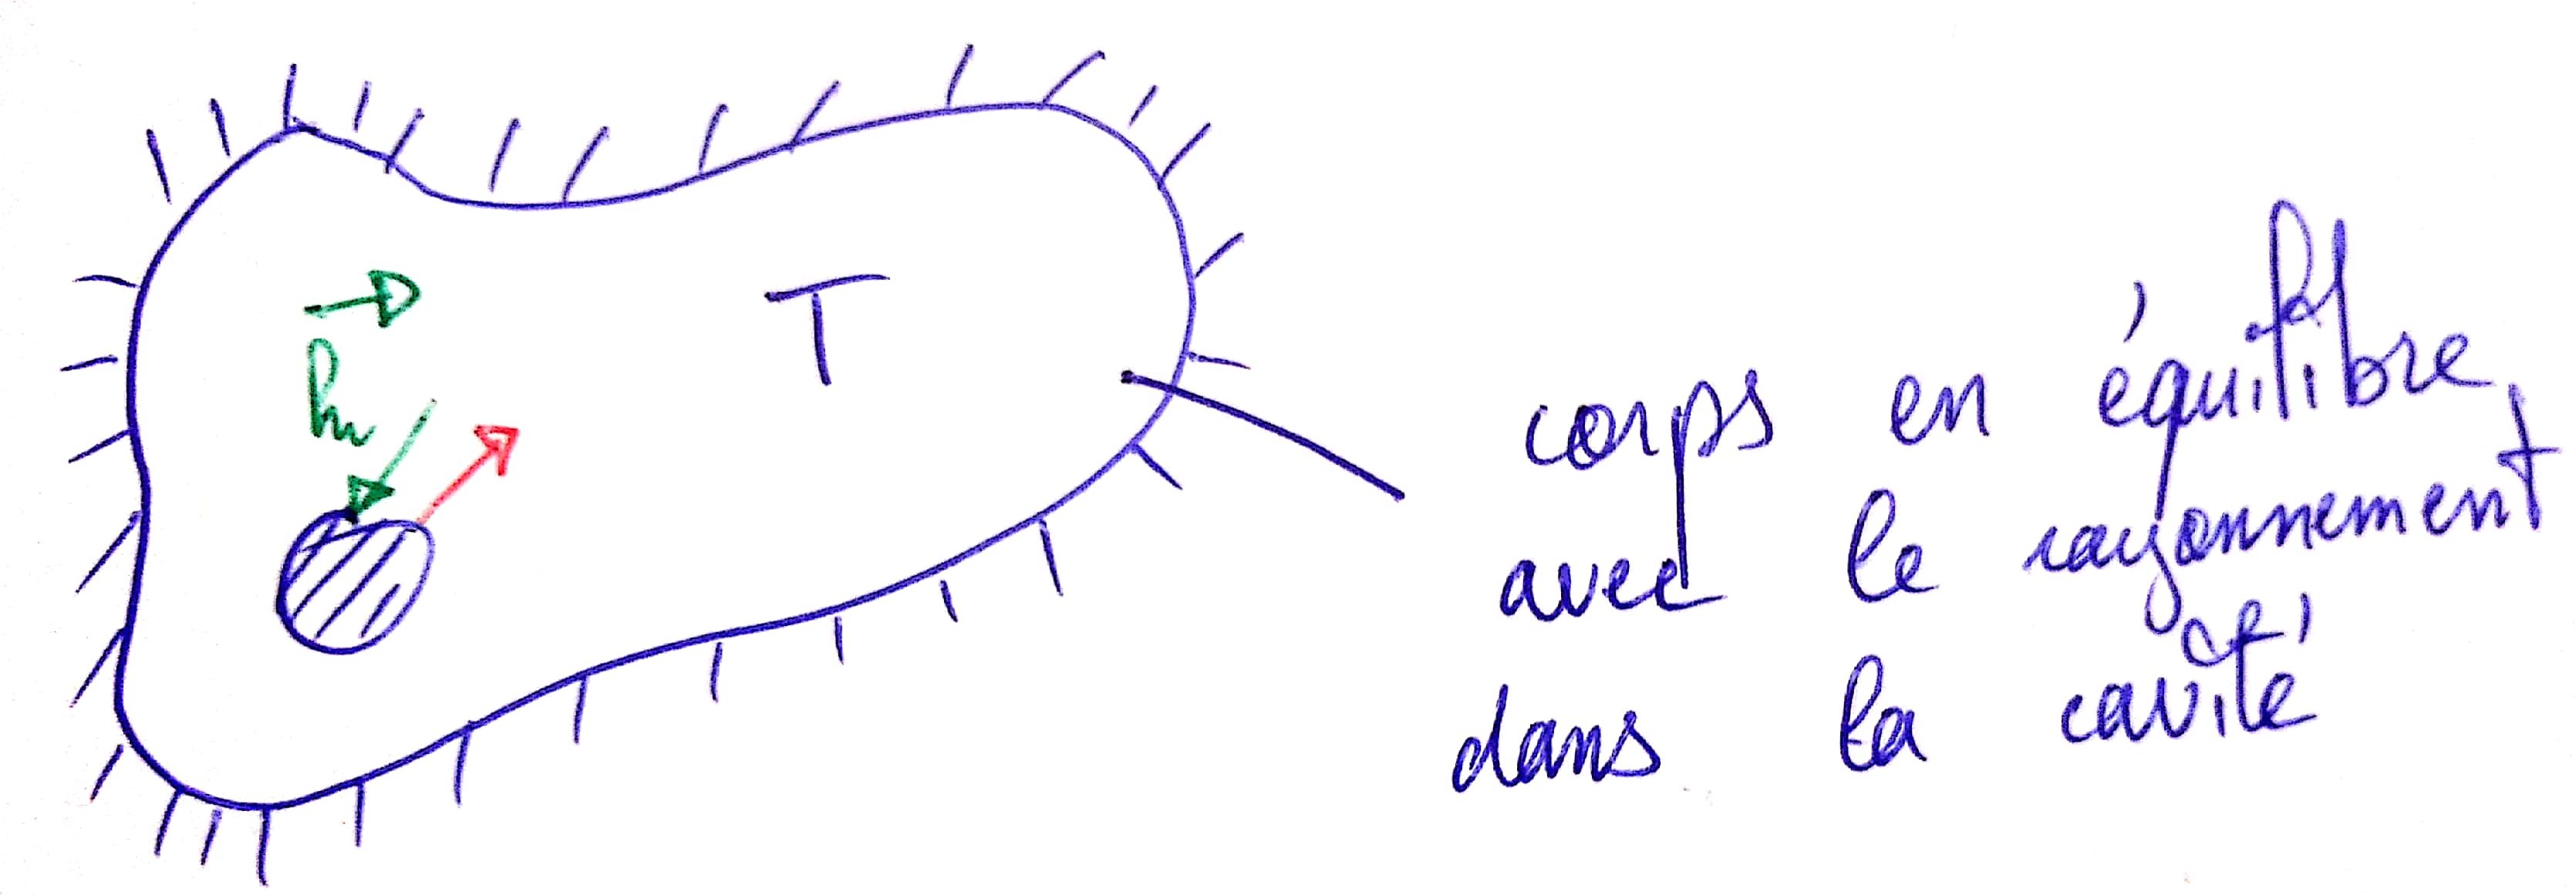
\includegraphics[width=10cm]{corps_noir}
\end{figure}


\textbf{Corps quelconque} : puissance émise par le corps = puissance absorbée.\\
Luminance :
\begin{eqnarray}
e_e(-\vec{k},\vec{\alpha}) = a(\vec{k},\vec{\alpha})e_i(\vec{k},\vec{\alpha})
\end{eqnarray}
$a(\vec{k},\vec{\alpha})$ facteur d'absorption.
$e_i(\vec{k},\vec{\alpha})$ : luminance incidente, indépendant du corps mais dépend de T.

\subsection{Corps noir}
C'est un cas particulier tel que $a(\vec{k},\vec{\alpha}) = 1\; \forall \vec{k}$ et $\forall \vec{\alpha}$, attention le quel que soit k signifie qu'on le voit noir dans tous les domaines, ceux qui nous apparaissent noir à nous on seulement $a(\vec{k},\vec{\alpha}) = 1$ dans le visible : "corps gris".

\section{Rayonnement de corps noir}
\textbf{Physique statistique} de \textit{B. Diu} chap VI partie III p818, \textbf{Physique statistique} de \textit{Couture et Zitoun} cahp 7 p195.
\subsection{Relier $e_i(\nu)$ à $u(\nu)$}
$u(\nu)$ est la densité spectrale d'énergie.
\begin{eqnarray}
U = \int dV \int d\nu\; u(\nu)
\end{eqnarray}
On fait le calcul de l'intégrale... on trouve $e(\nu) = \frac{c}{4}u(\nu)$

\subsection{Pression de radiation}
on calcule la pression de radiation (v livre de thermo).\\
On trouve 
\begin{equation}
pV = \frac{U}{3}
\end{equation}
On calcule ensuite 
\begin{eqnarray}
\left(\frac{\partial U}{\partial V}\right)_T = l-p = T\left(\frac{\partial p}{\partial T}\right)_V - p = p^3\\
\Rightarrow p \propto T^4
\end{eqnarray}

\subsection{Loi de Planck}
\begin{eqnarray}
u(\nu) = \frac{8\pi h}{c^3}\frac{\nu}{e^{h\nu/kT}-1}
\end{eqnarray}
La tracer. Commenter avec le fait qu'un four demeure noir tant qu'on ne dépasse pas une certaine température, au delà de cette température (environ 500°C) on voit apparaitre du rouge puis du orange (1200°C).

\subsection{Stefan Boltzmann}
On intègre $u(\nu)$ 

\begin{eqnarray}
\longrightarrow \varepsilon = \frac{c}{4} \int u(\nu) d\nu = \sigma T^4
\end{eqnarray}
très bien vérifié expérimentalement. Faire le lien avec le $T^4$ obtenu avant.

\subsection{Application}
On peut faire \\

\textbf{Thermodynamique} de \textit{B. Diu} p286.\\
Le soleil : photosphère à 5950 K. La puissance émise est $P = 4\pi R_{sol}^2\varepsilon$ et la puissance reçue sur terre à une distance d sur une surface S est 
\begin{eqnarray}
p = P\frac{S}{4\pi d^2} = S\left(\frac{R_{sol}}{d}\right)^2 \sigma T_{sol} ^4
\end{eqnarray}
on en déduit la température sur terre 
\begin{eqnarray}
T_T = T_{sol}\sqrt{\frac{R_{sol}}{2d}}
\end{eqnarray}	

ou sinon on peut faire le fond diffus cosmologique, plus dur et risqué, fait dans le Diu et le Zitoun.

\subsection{Démonstration de la loi de Planck}
\begin{eqnarray}
d^3N = 2\frac{d^3\vec{r}d^3\vec{p}}{h^3}\frac{1}{e^{\beta E}-1}
\end{eqnarray}
avec le facteur 2 pour les deux polarisations, et le facteur de Bose à droite. $\mu=0$ car nombre de photons conservés. 
\begin{eqnarray}
E = pc = h\nu\\
\int d^3\vec{r} = V\\
\int d\theta \sin\theta d\phi \rightarrow dN_{\nu} = \frac{8\pi V}{c^3}\frac{\nu^2d\nu}{e^{\beta\hbar\nu}-1}
\end{eqnarray}
\end{document}